% Importado desde: 2026-03-28_Causalidad_Efectiva_y_Cono_de_Luz_Emergente.tex
\chapter{Derivacion Pedagogica: --- causalidad efectiva y cono de luz emergente --- desde una dinamica discreta local}
\label{ch:causalidad-cono-luz}






% verified-by: validators/causality.py::test_group_velocity_diff_formula
% verified-by: validators/causality.py::test_massless_saturates_cone
% verified-by: validators/causality.py::test_group_velocity_strictly_below_v
% verified-by: validators/causality.py::test_lorentzian_signature
% verified-by: validators/causality.py::test_cone_determinant

\section{Objetivo}
En el capitulo anterior identificamos la \enquote{causalidad efectiva} como uno de los criterios decisivos para tomar en serio la idea de un espacio-tiempo emergente. La intuicion era clara, pero faltaba volverla mas precisa.

La pregunta concreta de este capitulo es:
\begin{displayquote}
\textbf{como aparece una velocidad maxima de propagacion en un modelo discreto local, y en que sentido esa velocidad induce un cono de luz efectivo?}
\end{displayquote}

Este paso es importante por dos razones:
\begin{enumerate}[label=\arabic*.]
    \item porque una geometria relativista no es solo un espectro lineal, sino tambien una organizacion causal de la propagacion;
    \item porque si queremos hablar de \enquote{proto-espacio-tiempo}, necesitamos una nocion estructural de \enquote{hasta donde puede influir algo en un tiempo dado}.
\end{enumerate}

\section{La idea fisica basica}
En una red discreta local, la informacion no puede saltar arbitrariamente lejos en un solo paso elemental de la dinamica. Esta restriccion ya sugiere una cota de propagacion.

\subsection{Que queremos mostrar}
Queremos justificar el siguiente esquema:
\begin{enumerate}[label=\arabic*.]
    \item la localidad microscopica restringe los saltos elementales;
    \item al iterar la dinamica, esa restriccion genera una region de influencia creciente pero finita;
    \item esa region define una velocidad maxima efectiva;
    \item en el sector infrarrojo isotropo, esa velocidad se interpreta como la velocidad limite del continuo efectivo.
\end{enumerate}

\begin{figure}[h!]
\centering
\begin{tikzpicture}[
    box/.style={draw, rounded corners, thick, align=center, minimum width=3.6cm, minimum height=1.1cm},
    arr/.style={-{Latex[length=3mm]}, thick}
]
\node[box, fill=blue!8] (a) at (0,0) {localidad\\microscopica};
\node[box, fill=green!8] (b) at (4.5,0) {velocidad\\maxima};
\node[box, fill=yellow!12] (c) at (9,0) {cono causal\\efectivo};
\node[box, fill=red!8] (d) at (13.5,0) {proto-geometria\\relativista};
\draw[arr] (a) -- (b);
\draw[arr] (b) -- (c);
\draw[arr] (c) -- (d);
\end{tikzpicture}
\caption{La logica conceptual que vamos a construir en este capitulo.}
\end{figure}

\section{Modelo microscopico minimo}
Tomemos una red cubica con espaciamiento \(a\). Para no mezclar demasiados ingredientes, pensemos en un Hamiltoniano local de tiempo continuo:
\begin{equation}
H = \sum_{\bm{n}} \psi_{\bm{n}}^\dagger M_0 \psi_{\bm{n}}
 + \sum_{\bm{n},\,i=1}^3
\left(
\psi_{\bm{n}}^\dagger T_i \psi_{\bm{n}+\hat{\imath}}
+ \psi_{\bm{n}+\hat{\imath}}^\dagger T_i^\dagger \psi_{\bm{n}}
\right),
\label{c19:eq:Hlocal}
\end{equation}
donde:
\begin{enumerate}[label=\arabic*.]
    \item \(\bm{n}\) recorre los sitios de la red;
    \item \(\psi_{\bm{n}}\) tiene varias componentes internas;
    \item \(M_0\) actua dentro de cada celda;
    \item \(T_i\) acopla solo primeros vecinos.
\end{enumerate}

Este es exactamente el tipo de estructura que hemos usado una y otra vez: \textit{tight-binding}, Wilson--Dirac, o bloques locales que luego linealizamos.

\subsection{La ecuacion de evolucion}
La dinamica de Schrodinger es
\begin{equation}
i\partial_t \ket{\Psi(t)} = H\ket{\Psi(t)},
\qquad
\ket{\Psi(t)} = e^{-iHt}\ket{\Psi(0)}.
\label{c19:eq:evol}
\end{equation}

La pregunta de causalidad es ahora muy concreta: si al tiempo \(t=0\) excitamos solo un sitio \(\bm{m}\), \textbf{cuanto tarda en aparecer amplitud apreciable en un sitio lejano \(\bm{n}\)?}

\section{Primer argumento: la potencia \(H^r\) no puede saltar mas de \(r\) enlaces}
Este es el corazon del argumento.

\subsection{Distancia de red}
Definamos la distancia Manhattan entre dos sitios como
\begin{equation}
d(\bm{n},\bm{m}) = \abs{n_x-m_x}+\abs{n_y-m_y}+\abs{n_z-m_z}.
\label{c19:eq:dist}
\end{equation}

Si el Hamiltoniano solo conecta primeros vecinos, entonces una aplicacion de \(H\) puede cambiar la posicion, como mucho, en una unidad de esta distancia.

\subsection{Consecuencia para potencias de \(H\)}
Por tanto:
\begin{equation}
\mel{\bm{n}}{H^r}{\bm{m}} = 0
\qquad
\text{si } d(\bm{n},\bm{m}) > r.
\label{c19:eq:Hrzero}
\end{equation}

\subsubsection*{Lectura fisica}
\begin{enumerate}[label=\arabic*.]
    \item \(H\) mueve a lo sumo un enlace;
    \item \(H^2\) mueve a lo sumo dos enlaces;
    \item \(H^r\) mueve a lo sumo \(r\) enlaces.
\end{enumerate}

Es una observacion simple, pero ya contiene la semilla del cono causal.

\begin{figure}[h!]
\centering
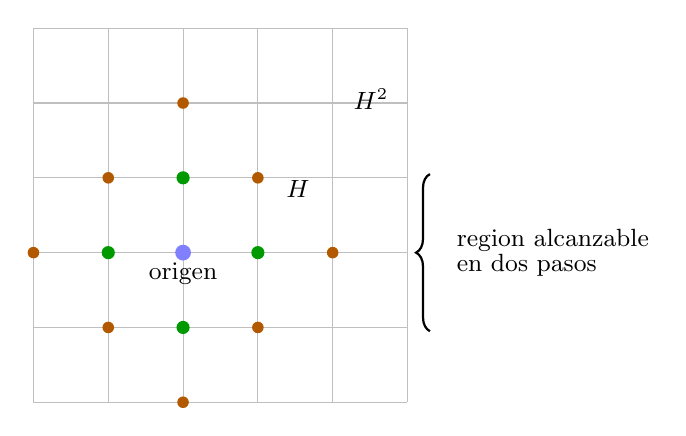
\begin{tikzpicture}[scale=0.95]
\foreach \x in {0,1,2,3,4,5}{
    \draw[gray!50] (\x,0) -- (\x,5);
    \draw[gray!50] (0,\x) -- (5,\x);
}
\fill[blue!50] (2,2) circle (3pt);
\foreach \p in {(2,3),(2,1),(1,2),(3,2)}{
    \fill[green!60!black] \p circle (2.5pt);
}
\foreach \p in {(2,4),(2,0),(0,2),(4,2),(1,3),(1,1),(3,3),(3,1)}{
    \fill[orange!70!black] \p circle (2.2pt);
}
\node[below] at (2,2) {\small origen};
\node[right] at (3.25,2.85) {\small \(H\)};
\node[right] at (4.15,4.05) {\small \(H^2\)};
\draw[decorate,decoration={brace,amplitude=5pt},thick]
    (5.3,0.95) -- (5.3,3.05)
    node[midway,right=6pt,align=left] {\small region alcanzable\\[-1mm]\small en dos pasos};
\end{tikzpicture}
\caption{Con primeros vecinos, \(H\) alcanza la primera corona y \(H^2\) alcanza la segunda.}
\end{figure}

\section{Segundo argumento: la serie temporal del propagador}
Expandamos el operador de evolucion:
\begin{equation}
U(t)=e^{-iHt}
= \sum_{r=0}^{\infty}\frac{(-it)^r}{r!}H^r.
\label{c19:eq:Useries}
\end{equation}

Tomemos el elemento matricial entre \(\bm{m}\) y \(\bm{n}\):
\begin{equation}
\mel{\bm{n}}{U(t)}{\bm{m}}
= \sum_{r=0}^{\infty}\frac{(-it)^r}{r!}\mel{\bm{n}}{H^r}{\bm{m}}.
\label{c19:eq:matrixel}
\end{equation}

Usando \eqref{c19:eq:Hrzero}, si \(L=d(\bm{n},\bm{m})\), los terminos con \(r<L\) desaparecen:
\begin{equation}
\mel{\bm{n}}{U(t)}{\bm{m}}
= \sum_{r=L}^{\infty}\frac{(-it)^r}{r!}\mel{\bm{n}}{H^r}{\bm{m}}.
\label{c19:eq:tailseries}
\end{equation}

\subsection{La consecuencia inmediata}
Para que aparezca amplitud en un punto a distancia \(L\), la evolucion necesita acumular suficientes potencias de \(H\). En tiempos muy cortos, esto fuerza una fuerte supresion.

\subsection{Cota sencilla}
Si \(\norm{H}\) denota la norma operatorial, entonces
\begin{equation}
\abs{\mel{\bm{n}}{H^r}{\bm{m}}}\le \norm{H}^r,
\end{equation}
y por tanto
\begin{equation}
\abs{\mel{\bm{n}}{U(t)}{\bm{m}}}
\le
\sum_{r=L}^{\infty}\frac{(\norm{H}t)^r}{r!}.
\label{c19:eq:tailbound}
\end{equation}

Para \(L>\norm{H}t\), esta cola factorial cae rapidamente. Una cota pedagogica util es
\begin{equation}
\sum_{r=L}^{\infty}\frac{x^r}{r!}
\le
e^x\left(\frac{ex}{L}\right)^L,
\qquad x=\norm{H}t.
\label{c19:eq:factorialbound}
\end{equation}

Luego:
\begin{equation}
\abs{\mel{\bm{n}}{U(t)}{\bm{m}}}
\lesssim
e^{\norm{H}t}\left(\frac{e\norm{H}t}{L}\right)^L.
\label{c19:eq:finalbound}
\end{equation}

\subsection{Que significa la cota}
Si la distancia de red \(L\) es mucho mayor que \(e\norm{H}t\), la amplitud queda exponencialmente suprimida. Esto no dice que sea exactamente cero, pero si dice algo muy fuerte:
\begin{displayquote}
\textbf{fuera de una region aproximadamente lineal en el tiempo, la propagacion esta drasticamente suprimida.}
\end{displayquote}

Esta es la estructura conceptual de una cota tipo Lieb--Robinson, aunque aqui la estamos presentando en una version pedagogica y no en su forma matematica mas general.

\section{Aparicion de una velocidad maxima}
La distancia fisica es \(r=aL\). Si la frontera efectiva aparece cuando \(L\sim e\norm{H}t\), entonces:
\begin{equation}
r \sim a\,e\norm{H}\, t.
\end{equation}

Esto sugiere una velocidad maxima microscopica del orden
\begin{equation}
v_{\text{micro}} \sim a\,e\norm{H}.
\label{c19:eq:vmicro}
\end{equation}

\subsection{Interpretacion correcta}
No debemos obsesionarnos aqui con el factor numerico exacto. Lo importante es la estructura:
\begin{enumerate}[label=\arabic*.]
    \item la localidad microscopica produce una cota lineal en el tiempo;
    \item esa cota define una velocidad maxima de propagacion;
    \item por debajo de esa frontera la dinamica puede ser apreciable;
    \item muy por fuera de ella la influencia queda exponencialmente pequena.
\end{enumerate}

\begin{figure}[h!]
\centering
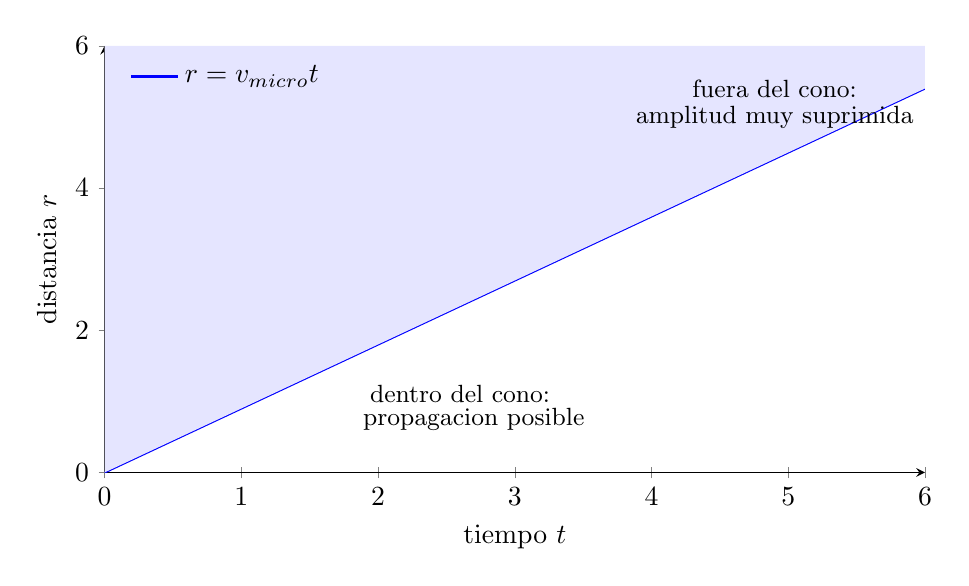
\begin{tikzpicture}
\begin{axis}[
    width=12cm,
    height=7cm,
    xlabel={tiempo \(t\)},
    ylabel={distancia \(r\)},
    xmin=0, xmax=6,
    ymin=0, ymax=6,
    axis lines=left,
    samples=2,
    domain=0:6,
    legend style={draw=none, fill=none, at={(0.02,0.98)}, anchor=north west}
]
\addplot[thick, blue] {0.9*x};
\addlegendentry{\(r=v_{\text{micro}}t\)}
\fill[blue!10] (axis cs:0,0) -- (axis cs:6,5.4) -- (axis cs:6,6) -- (axis cs:0,6) -- cycle;
\node at (axis cs:4.9,5.4) {\small fuera del cono:};
\node at (axis cs:4.9,5.0) {\small amplitud muy suprimida};
\node at (axis cs:2.6,1.1) {\small dentro del cono:};
\node at (axis cs:2.7,0.75) {\small propagacion posible};
\end{axis}
\end{tikzpicture}
\caption{La localidad induce una region de influencia aproximadamente conica en el plano espacio-tiempo efectivo.}
\end{figure}

\section{Del cono microscopico al cono relativista efectivo}
Hasta aqui solo hemos mostrado una velocidad maxima nacida de la localidad. Ahora hay que conectarla con la velocidad del sector Dirac isotropo.

\subsection{Hamiltoniano efectivo}
En el subsector infrarrojo tenemos
\begin{equation}
H_{\text{eff}}(\bm{q}) = v\,\bm{\alpha}\cdot\bm{q} + m\beta,
\label{c19:eq:Heff}
\end{equation}
con dispersion
\begin{equation}
E(\bm{q})=\pm\sqrt{m^2+v^2\abs{\bm{q}}^2}.
\label{c19:eq:dispdirac}
\end{equation}

\subsection{Velocidad de grupo}
La velocidad de grupo es
\begin{equation}
\bm{v}_g = \nabla_{\bm{q}} E(\bm{q})
= \pm \frac{v^2 \bm{q}}{\sqrt{m^2+v^2\abs{\bm{q}}^2}}.
\label{c19:eq:vg}
\end{equation}

Su modulo satisface
\begin{equation}
\abs{\bm{v}_g}
=
\frac{v^2\abs{\bm{q}}}{\sqrt{m^2+v^2\abs{\bm{q}}^2}}
\le v.
\label{c19:eq:vgbound}
\end{equation}

\subsection{Lectura fisica}
El continuo efectivo trae su propia velocidad limite, que es precisamente \(v\), la velocidad del cono de Dirac. Luego aparecen dos escalas:
\begin{enumerate}[label=\arabic*.]
    \item una velocidad microscopica \(v_{\text{micro}}\) impuesta por la localidad de la red;
    \item una velocidad efectiva \(v\) que controla la cinematica relativista infrarroja.
\end{enumerate}

Para que la interpretacion geometrica sea limpia, queremos que estas dos estructuras sean compatibles.

\section{La condicion de compatibilidad}
La condicion minima es:
\begin{equation}
v \le v_{\text{micro}}.
\label{c19:eq:compat}
\end{equation}

\subsection{Por que}
Si el sector Dirac predijera paquetes de onda con velocidad mayor que la permitida por la microdinamica, entonces el continuo efectivo seria inconsistente con el modelo subyacente.

\subsection{Lo que idealmente queremos}
Idealmente, no solo queremos \eqref{c19:eq:compat}. Queremos ademas que:
\begin{enumerate}[label=\arabic*.]
    \item el cono infrarrojo este bien contenido en el cono microscopico;
    \item las correcciones de red deformen ese cono solo a orden alto;
    \item la isotropia del sector Dirac sobreviva a escalas suficientemente grandes.
\end{enumerate}

\begin{figure}[h!]
\centering
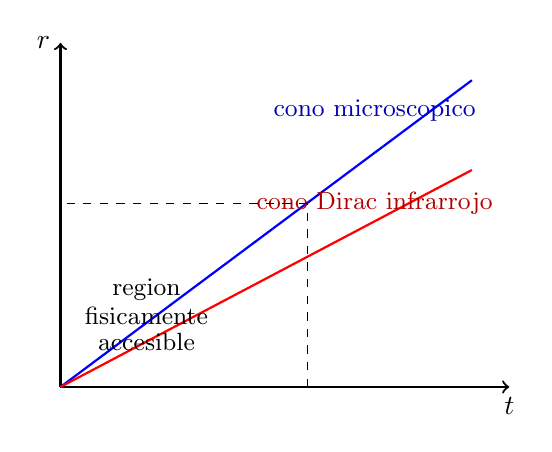
\begin{tikzpicture}[scale=0.95]
\draw[->, thick] (0,0) -- (0,4.6) node[left] {\(r\)};
\draw[->, thick] (0,0) -- (6,0) node[below] {\(t\)};
\draw[thick, blue] (0,0) -- (5.5,4.1);
\draw[thick, red] (0,0) -- (5.5,2.9);
\node[blue!70!black] at (4.2,3.7) {\small cono microscopico};
\node[red!70!black] at (4.2,2.45) {\small cono Dirac infrarrojo};
\draw[dashed] (3.3,0) -- (3.3,2.45);
\draw[dashed] (3.3,2.45) -- (0,2.45);
\node at (1.15,1.3) {\small region};
\node at (1.15,0.95) {\small fisicamente};
\node at (1.15,0.6) {\small accesible};
\end{tikzpicture}
\caption{El cono efectivo de Dirac debe ser compatible con la velocidad maxima impuesta por la microdinamica.}
\end{figure}

\section{Un comentario importante sobre isotropia}
La existencia de velocidad maxima no basta por si sola para hablar de espacio-tiempo emergente. Tambien importa la forma del frente de propagacion.

\subsection{Caso anisotropo}
Si el sector efectivo fuera
\begin{equation}
E^2 \simeq m^2 + v_x^2 q_x^2 + v_y^2 q_y^2 + v_z^2 q_z^2,
\end{equation}
entonces la region causal infrarroja estaria deformada.

\subsection{Caso isotropo}
En cambio, cuando
\begin{equation}
E^2 \simeq m^2 + v^2\abs{\bm{q}}^2,
\end{equation}
el frente de propagacion de baja energia es isotropo y la interpretacion como metrica efectiva se vuelve mucho mas natural.

Por eso el sector Dirac isotropo sigue siendo el punto base correcto del proyecto.

\section{Que cambia en tiempo discreto}
El caso de \textit{quantum walks} y \textit{QCA} es aun mas sugerente.

\subsection{Paso elemental}
Si la dinamica avanza en pasos temporales \(\Delta t\) y en cada paso la excitacion puede desplazarse, como mucho, una distancia \(a\), entonces tras \(N\) pasos:
\begin{equation}
r \le Na.
\end{equation}

Como \(t=N\Delta t\), esto da
\begin{equation}
r \le \frac{a}{\Delta t} t.
\label{c19:eq:qwspeed}
\end{equation}

\subsection{Diferencia conceptual}
Aqui el cono causal puede ser exacto:
\begin{enumerate}[label=\arabic*.]
    \item fuera de la region permitida no hay solo supresion;
    \item directamente no existe soporte.
\end{enumerate}

Eso hace que los modelos con tiempo discreto sean especialmente atractivos para una lectura de espacio-tiempo emergente, porque la nocion de causalidad esta incorporada de manera mas elemental.

\begin{figure}[h!]
\centering
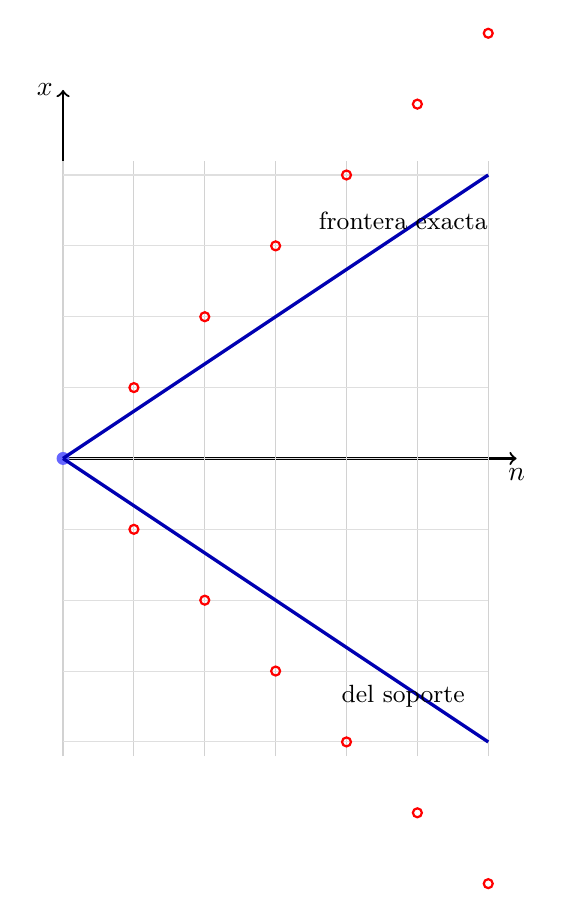
\begin{tikzpicture}[scale=0.9]
\draw[->, thick] (0,0) -- (0,5.2) node[left] {\(x\)};
\draw[->, thick] (0,0) -- (6.4,0) node[below] {\(n\)};
\foreach \n in {0,1,2,3,4,5,6}{
    \draw[gray!35] (\n,-4.2) -- (\n,4.2);
}
\foreach \x in {-4,-3,-2,-1,0,1,2,3,4}{
    \draw[gray!25] (0,\x) -- (6,\x);
}
\fill[blue!60] (0,0) circle (2.6pt);
\foreach \n/\m in {1/1,2/2,3/3,4/4,5/5,6/6}{
    \draw[thick, red] (\n,\m) circle (1.8pt);
    \draw[thick, red] (\n,-\m) circle (1.8pt);
}
\draw[very thick, blue!70!black] (0,0) -- (6,4);
\draw[very thick, blue!70!black] (0,0) -- (6,-4);
\node at (4.8,3.35) {\small frontera exacta};
\node at (4.8,-3.35) {\small del soporte};
\end{tikzpicture}
\caption{En una caminata cuantica con desplazamiento maximo por paso, el cono causal puede ser exacto.}
\end{figure}

\section{Que hemos ganado conceptualmente}
Ahora ya podemos reformular mejor el criterio de causalidad:
\begin{displayquote}
\textbf{un candidato razonable de proto-espacio-tiempo debe poseer una dinamica local cuya propagacion admita una velocidad maxima estructural y, en el sector infrarrojo, esa velocidad debe organizarse de forma compatible con el cono de Dirac efectivo.}
\end{displayquote}

\subsection{Lo que este capitulo aclara}
\begin{enumerate}[label=\arabic*.]
    \item la causalidad efectiva no sale de la nada; nace de la localidad;
    \item el cono relativista efectivo no reemplaza al cono microscopico, sino que emerge dentro de el;
    \item la isotropia infrarroja es crucial para interpretar esa estructura como geometria;
    \item el tiempo discreto ofrece una version aun mas fuerte de causalidad elemental.
\end{enumerate}

\section{Lo que ya podemos afirmar}
Con el trabajo acumulado hasta aqui, ya podemos decir con bastante seguridad:
\begin{enumerate}[label=\arabic*.]
    \item el modelo discreto local no permite propagacion arbitrariamente rapida;
    \item existe una velocidad maxima microscopica asociada a la localidad;
    \item el sector Dirac isotropo tiene su propia velocidad limite \(v\);
    \item la interpretacion cinematica como cono de luz efectivo empieza a ser seria cuando ambas estructuras son compatibles.
\end{enumerate}

\section{Lo que aun falta}
Todavia faltan dos pasos importantes.

\subsection{Primero}
Dar una formulacion mas rigurosa, ya no solo pedagogica, en terminos de observables locales y conmutadores, del estilo de las cotas de Lieb--Robinson.

\subsection{Segundo}
Comparar de forma sistematica dos estrategias:
\begin{enumerate}[label=\arabic*.]
    \item tiempo continuo con Hamiltoniano local;
    \item tiempo discreto con evolucion unitaria local tipo QW/QCA.
\end{enumerate}

Ese contraste es importante porque puede decirnos cual de las dos rutas ofrece una base mas natural para una interpretacion de espacio-tiempo emergente.

\section{Mapa del siguiente paso}
Si seguimos la ruta del proyecto sin perder el hilo, el siguiente paso natural es:
\begin{displayquote}
\textbf{comparar, con el mismo cuidado paso a paso, la causalidad emergente en el esquema Hamiltoniano de tiempo continuo con la causalidad exacta o cuasi-exacta de los modelos de tiempo discreto tipo quantum walk y QCA.}
\end{displayquote}

\begin{figure}[h!]
\centering
\begin{tikzpicture}[
    box/.style={draw, rounded corners, thick, align=center, minimum width=4cm, minimum height=1.1cm},
    arr/.style={-{Latex[length=3mm]}, thick}
]
\node[box, fill=blue!7] (a) at (0,0) {localidad de red};
\node[box, fill=green!7] (b) at (4.8,0) {velocidad maxima\\microscopica};
\node[box, fill=yellow!12] (c) at (9.6,0) {cono Dirac\\infrarrojo};
\node[box, fill=red!7] (d) at (14.4,0) {comparacion\\tiempo continuo / discreto};
\draw[arr] (a) -- (b);
\draw[arr] (b) -- (c);
\draw[arr] (c) -- (d);
\end{tikzpicture}
\caption{Este capitulo fija la base cinemática para la comparacion posterior entre tiempo continuo y tiempo discreto.}
\end{figure}

\section{Resumen final}
El punto central del capitulo es que la idea de un \enquote{cono de luz efectivo} no es una metafora libre, sino una consecuencia bastante natural de la localidad microscopica. En un Hamiltoniano de red local, las potencias de \(H\) solo pueden propagar amplitud paso a paso, y la serie temporal del propagador muestra que la influencia fuera de una region lineal en el tiempo queda fuertemente suprimida. Esa estructura induce una velocidad maxima microscopica.

Cuando ademas existe un sector Dirac isotropo, aparece una segunda velocidad, la velocidad \(v\) del continuo efectivo. El proyecto gana fuerza precisamente cuando ambas velocidades son compatibles y cuando el frente infrarrojo es isotropo. En ese punto empezamos a tener, no todavia un espacio-tiempo completo, pero si una base cinemática razonable para hablar de proto-causalidad y de pregeometria emergente.
